\section{\textbf{Evaluation}}\label{sec:5}

	First of all the breadboard circuit (Figure~\ref{fig:proto_h}) was tested using a multimeter to ensure it's proper functionality. With Q1 and Q2 activated the voltage measured across the motor was $3.5\;V$, for future analysis this situation (Q1 and Q2 active) will be called S1. With Q3 and Q4 activated the voltage measured was $-2.6\;V$, this will be the S2 situation. The polarity inversion was accomplished, however the magnitude for both cases which was expected to be equal was in fact different. A slightly tension drop occurred when the current flew backwards. One important thing to mention is that when the transistor is turned off (base voltage = 0) it's output is not exactly equals zero, it shows a remainder voltage of $0.6\;V$ however this tension is not enough to move the motor.
	
	Despite the previous mentioned discrepancy, which solution will be discussed later on the circuit performed as intentioned therefore the motor was plugged into the circuit. For S1 the motor spun in the counterclockwise direction. On the other hand for S2 it spun clockwise slightly slower, as a result of the voltage drop previous mentioned.
	
	Finally with the printed circuit board in hands the tension across the output pins were once again measured with a voltmeter. In case S1 the voltage showed up to be $3.6\;V$ which is equal to the breadboard circuit, the same occurred for S2. As the PCB performed exactly as the breadboard circuit the motor was connected and the final configuration version 1 was achieved.
	
	In order to achieve a better performance and eliminate the previous mentioned tension drop for S2 this configuration needed to change a bit. A possible cause for this issue was a remaining current when the transistor should be turned off. Hence four resistors were added between the transistor's base resistor and the ground node (see Figure~\ref{fig:h_schem_v2}. The intention of this change is to force any remaining current flows to the ground node.
	
	The final configuration version 2 filled the expectations. For S1 case the tension across the motor was $3.84\;V$. And now for S2 case the tension showed to be $-3.78\;V$ which result in equal spin velocity for both cases.
	
\begin{figure}[b]
\centering
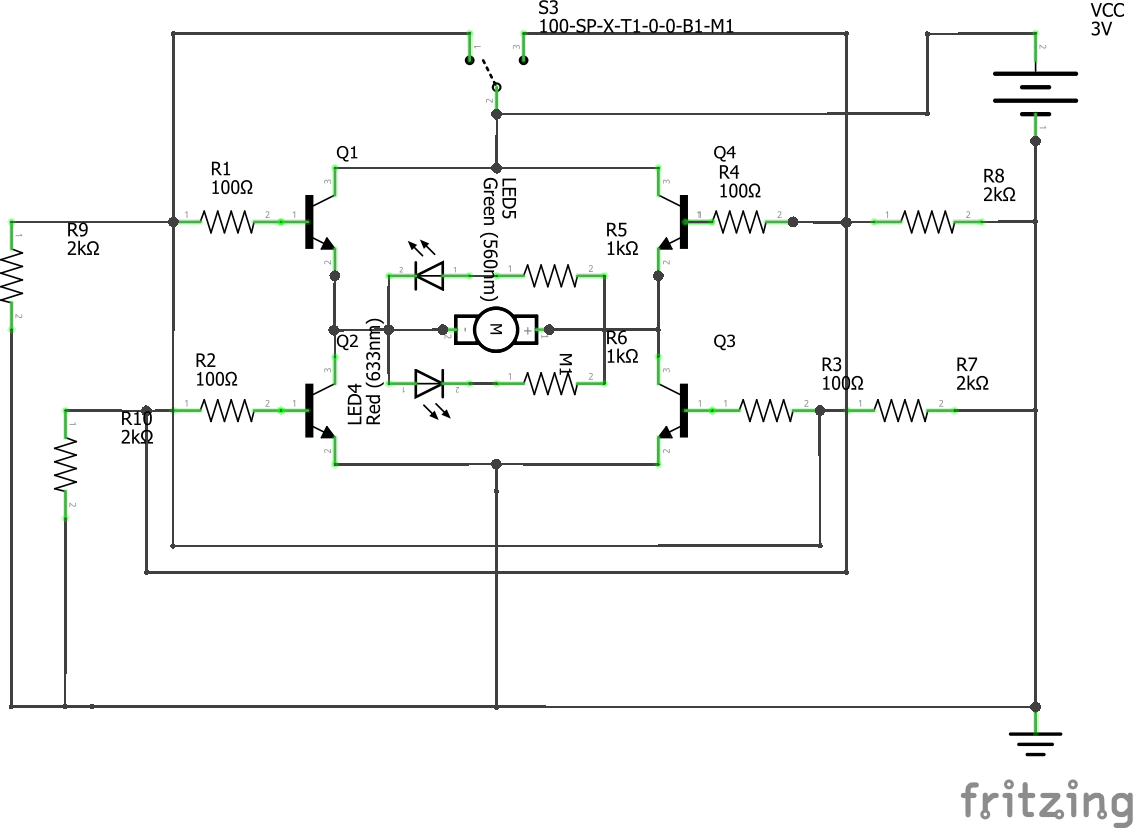
\includegraphics[width=\columnwidth]{img/ponteH_schem_new.png}
\caption{Final configuration version 2 schematic.}
\label{fig:h_schem_v2}
\end{figure}

